%%%%%%%%%%%%%%%%%%%%%%% file template.tex %%%%%%%%%%%%%%%%%%%%%%%%%
%
% This is a general template file for the LaTeX package SVJour3
% for Springer journals.          Springer Heidelberg 2010/09/16
%
% Copy it to a new file with a new name and use it as the basis
% for your article. Delete % signs as needed.
%
% This template includes a few options for different layouts and
% content for various journals. Please consult a previous issue of
% your journal as needed.
%
%%%%%%%%%%%%%%%%%%%%%%%%%%%%%%%%%%%%%%%%%%%%%%%%%%%%%%%%%%%%%%%%%%%
%
% First comes an example EPS file -- just ignore it and
% proceed on the \documentclass line
% your LaTeX will extract the file if required
% \begin{filecontents*}{example.eps}
% %!PS-Adobe-3.0 EPSF-3.0
% %%BoundingBox: 19 19 221 221
% %%CreationDate: Mon Sep 29 1997
% %%Creator: programmed by hand (JK)
% %%EndComments
% gsave
% newpath
%   20 20 moveto
%   20 220 lineto
%   220 220 lineto
%   220 20 lineto
% closepath
% 2 setlinewidth
% gsave
%   .4 setgray fill
% grestore
% stroke
% grestore
% \end{filecontents*}
%
\RequirePackage{fix-cm}

%
%\documentclass[natbib]{svjour3}                     % onecolumn (standard format)
%\documentclass[natbib,smallcondensed]{svjour3}     % onecolumn (ditto)
\documentclass[natbib,smallextended]{svjour3}\usepackage[]{graphicx}\usepackage[]{color}
%% maxwidth is the original width if it is less than linewidth
%% otherwise use linewidth (to make sure the graphics do not exceed the margin)
\makeatletter
\def\maxwidth{ %
  \ifdim\Gin@nat@width>\linewidth
    \linewidth
  \else
    \Gin@nat@width
  \fi
}
\makeatother

\definecolor{fgcolor}{rgb}{0.345, 0.345, 0.345}
\newcommand{\hlnum}[1]{\textcolor[rgb]{0.686,0.059,0.569}{#1}}%
\newcommand{\hlstr}[1]{\textcolor[rgb]{0.192,0.494,0.8}{#1}}%
\newcommand{\hlcom}[1]{\textcolor[rgb]{0.678,0.584,0.686}{\textit{#1}}}%
\newcommand{\hlopt}[1]{\textcolor[rgb]{0,0,0}{#1}}%
\newcommand{\hlstd}[1]{\textcolor[rgb]{0.345,0.345,0.345}{#1}}%
\newcommand{\hlkwa}[1]{\textcolor[rgb]{0.161,0.373,0.58}{\textbf{#1}}}%
\newcommand{\hlkwb}[1]{\textcolor[rgb]{0.69,0.353,0.396}{#1}}%
\newcommand{\hlkwc}[1]{\textcolor[rgb]{0.333,0.667,0.333}{#1}}%
\newcommand{\hlkwd}[1]{\textcolor[rgb]{0.737,0.353,0.396}{\textbf{#1}}}%

\usepackage{framed}
\makeatletter
\newenvironment{kframe}{%
 \def\at@end@of@kframe{}%
 \ifinner\ifhmode%
  \def\at@end@of@kframe{\end{minipage}}%
  \begin{minipage}{\columnwidth}%
 \fi\fi%
 \def\FrameCommand##1{\hskip\@totalleftmargin \hskip-\fboxsep
 \colorbox{shadecolor}{##1}\hskip-\fboxsep
     % There is no \\@totalrightmargin, so:
     \hskip-\linewidth \hskip-\@totalleftmargin \hskip\columnwidth}%
 \MakeFramed {\advance\hsize-\width
   \@totalleftmargin\z@ \linewidth\hsize
   \@setminipage}}%
 {\par\unskip\endMakeFramed%
 \at@end@of@kframe}
\makeatother

\definecolor{shadecolor}{rgb}{.97, .97, .97}
\definecolor{messagecolor}{rgb}{0, 0, 0}
\definecolor{warningcolor}{rgb}{1, 0, 1}
\definecolor{errorcolor}{rgb}{1, 0, 0}
\newenvironment{knitrout}{}{} % an empty environment to be redefined in TeX

\usepackage{alltt}   % onecolumn (second format)
%\documentclass[twocolumn]{svjour3}          % twocolumn
%
\smartqed  % flush right qed marks, e.g. at end of proof
%
\usepackage{graphicx}
\usepackage[section]{placeins}
\usepackage{hyperref}
\usepackage{amsmath}


%
% \usepackage{mathptmx}      % use Times fonts if available on your TeX system
%
% insert here the call for the packages your document requires
%\usepackage{latexsym}
% etc.
%
% please place your own definitions here and don't use \def but
% \newcommand{}{}
%
% Insert the name of "your journal" with
\journalname{Review of Economics of the Household}
%
\IfFileExists{upquote.sty}{\usepackage{upquote}}{}
\begin{document}

\title{Constrained Parenting Decisions%\thanks{Grants or other notes
%about the article that should go on the front page should be
%placed here. General acknowledgments should be placed at the end of the article.}
}
\subtitle{Toward a General Model of Child Maltreatment}

%\titlerunning{Short form of title}        % if too long for running head

\author{Joseph A. Mienko}

%\authorrunning{Short form of author list} % if too long for running head


\institute{J. Mienko \at
              University of Washington Box 359476 \\
              Seattle, WA 98195 \\
              Tel.: +1-253-514-3632\\
              \email{mienkoja@uw.edu}           %  \\
}

\date{Received: date / Accepted: date}
% The correct dates will be entered by the editor


\maketitle

\begin{abstract}
Standard parental investment models from the biological sciences and economics suggest that parents can be expected to care for their children subject to personal characteristics (e.g. altruism) and resource constraints (e.g. money). While previous research has clearly established links between personal characteristics, resources, and maltreatment behaviors, the field lacks any examples of formal attempts to test the predictions of these models with respect to maltreatment behaviors. The goal of this paper is to test a biologically and economically informed model of behaviors associated with child maltreatment. Using data from the National Survey of Early Childhood Health (NSECH), the Consumer Expenditure Survey (CES), and the American Time Use Survey (ATUS), estimates of altruism, parental efficiency, income, and other control variables were calculated. A dependent measure of the probability that all reported discipline strategies would be Type-II strategies was also calculated. All variables were subjected to Bayesian Model Averaging (BMA) across quasibinomial GLMs to determine the most probable set of covariates. The BMA results estimate that the model with the highest posterior probability is a model which only includes the household and parental investments (household altruism) and the natural logarithm of their annual income. In other words, households with higher levels of altruism and higher incomes tend to report higher levels of discipline strategies that are not associated with maltreatment. Results are discussed in terms of implications for social work practice and child welfare practice in particular. 

\keywords{Income\and Altruism\and Child maltreatment\and Child Abuse\and Child Neglect\and Discipline}
% \PACS{PACS code1 \and PACS code2 \and more}
\subclass{91 \and 92}
\end{abstract}

\section{Introduction}
\label{intro}
A relatively underdeveloped area of household economic literature concerns the manner in which the maltreatment of children is formally understood or modeled. This deficit is due, at least in part, to the general perception that child maltreatment is best conceptualized as an irrational or even pathological act. Such perceptions are well-documented by \citet{Nelson1986} who notes that modern conceptions of child maltreatment have been largely framed by the medical community which defines the problem of child maltreatment imprecisely in terms of social deviance and a defect in the character of parents who engage in maltreatment. 

The central thesis of this paper is that maltreatment can be conceptualized as the non-pathological consequence of parenting under resource constraints. All parenting behavior (even maltreative\footnote{Here, the word ``maltreative'' is used, as an adjective describing care which is characterized by violence or neglect without regard to malice. Such an adjective is important for the framework presented in this manuscript in order to avoid categorization of behaviors by way of adjectives such as ``abusive'' or ``neglectful'' while also avoiding the inherent presence of malice in the use of an adjective such as ``malicious''. While other candidate adjectives exist (e.g. \emph{laesive} from the Latin adjective \emph{laesus} meaning injured), ``maltreative'' is chosen due to the relative semantic comfort that most of this manuscript's probable readership will find with this word.} parenting behavior) can be reduced to decisions about how a parent chooses to invest their time and other resources in a given child. Under certain sets of resource constraints \emph{any} parent can be expected to engage in parenting decisions that society would tend to judge as maltreative. While child maltreatment may be undesirable, in most cases it is not pathological. Recognition of this basic distinction has important implications for child welfare policy and practice.

\subsection{Brief Overview of Maltreatment Literature}

The basic relationship between resources and child maltreatment is well-established in non-economic social science literature with previous studies establishing links between resource constraints and substantiated allegations of child maltreatment as well as general involvement with the child welfare system \citep{Gil1970, Pelton1981, Pelton1994, Russell1984, Sedlak1996, Stith2009, BergerAndWoldfogel2004}. Studies examining administrative data sets of low-income populations (e.g. TANF recipients) have also shown that exogenous resource-decreasing shocks such as welfare-reform \citep{Courtney2005} or welfare sanctions \citep{Slack2007} will tend to increase a family's probability of child welfare system involvement. Other studies have exploited experimental income support programs to address income endogeneity problems inherent in other studies and still find an inverse relationship between family income and the probability of child maltreatment \citep{Cancian2013, Fein2003}. While there is a paucity of research examining connections between income and child maltreatment outside of the US \citep{Cameron2006}, the evidence from the US seems to suggest a strong and reliable relationship between child welfare system involvement and resource levels. 

While the literature provides multiple examples of research establishing a link between resources constraints and child maltreatment, the field is lacking in attempts to formally specify a mechanism to explain this relationship. Two exceptions to this rule include \citet{Brandon1999} and \citet{Brandon2001}. In each of these studies, microeconomic models are proposed which outline the manner in which parental resource constraints can lead to maltreatment. The former study suggests that maltreatment is mainly effected by a parent's level of altruism, the latter suggests that maltreatment is a function of how efficiently a parent uses her available resources. Both effects are viewed as subject to income constraints. In this paper, a variation on these models is proposed followed by an attempt to test key predictions of the model. 

\section{Maltreatment from Biological Altruism}
\label{bio_altruism}

\subsection{Hamilton's Rule}

While a full review of the nature vs. nurture debate is beyond the scope of this manuscript, this discussion proceeds from an assumption that human beings are simultaenously biological \emph{and} social beings \citep[see for example][]{Plomin1994, Ridley2003}. In other words, human beings are not born as a \emph{tabula rasa}. Humans are born endowed with tendencies to engage in certain activities such as learning languages, consuming nutrients, and engaging in bipedal locomotion. These activities are certainly moderated by the environment in which a human finds himself, but there is no doubt that human genetic makeup helps humans to engage in these activities regardless of an individual's environmental circumstances. Basic evolutionary theory demonstrates that such behaviors exist \emph{because} they helped human genes to evolve to their present state. 

One type of behavior that enabled human genes to survive is parenting behavior and parental altruism in particular. As described in such seminal works as \citet{Hamilton1964} and \citet{Trivers1974}, parental altruism can be defined as those behaviors requiring the investment of time or other resources in a child in a way that benefits the child (in terms of her fitness as a future mate) but comes at a cost to the parent (in terms of her fitness as a future mate). This does not preclude the parent from receiving some sort of benefit from the altruistic act. \citet{Stuebe2010}, for example, find that breastfeeding decreases a mother's long term risk of developing certain chronic diseases. To the extent that an increased survival probability would allow a mother to produce more offspring, she can be viewed as benefiting from the activity to some extent. However, when considering the costs associated with breastfeeding (in terms of caloric loss, the opportunity cost of not bearing other children, etc.), there may be a net cost to the \emph{mother's} long term fitness but a gain in the probability that her genes are spread \emph{into the population as a whole}. In such situations, parental behavior is said to be altruistic.

\citet{Hamilton1964} has shown that such altruistic tendencies can, themselves, be conceptualized as genetic traits. Hamilton establishes further that such altruistic tendencies will spread in a population subject to the constraint 
\begin{equation}
rb > c
\end{equation}
where $b$ indicates the benefit gained from an altruistic act (in terms of gene survival probability), $c$ indicates the associated cost of the act and $r$ indicates the relatedness parameter which specifies the proportion of genes that the recipient of an altruistic act shares in common with the individual performing the act. For simplicity, this paper focuses only on households and the altruistic acts of parents for their own children. As such, we can treat the constraint as simply 
\begin{equation}
b > c.
\end{equation}
The above constraint specifies that parents will not act altruistically toward their children beyond the point at which benefits outweigh the costs of the altruistic act in terms of gene survival. While there are many situtations in which this constraint can be violated (thus causing a parent to tend toward non-altruistic acts). One of the most obvious is a situation in which we assume a fixed level of resources for a parent. The increase in gene survival probability obtained from an altruistic act is dependent on the available resources to a parent. This is because when a parent makes a choice to invest in one child, they are necessarily making a choice to not invest in their other children (or their future children). Thus, under extremely low levels of fixed resources the marginal gain in survival probability for an investment in a given child may be so low that the parent chooses to invest in other (perhaps healthier) children or to simply reserve their resources for other children in a future state in which resources may be more abundant. In other words, parents can be expected to engage in triaging activities. 

\subsection{Triaging Activities}

Under periods of extreme scarcity, animals (and humans) will reliably engage in triaging activities in which they will fail to invest in children if it appears likely that investments in that child will come at the expense of another child more likely to survive the scarcity (including future children). This point is well articulated in \citet{Chagnon1983} where Chagnon's fieldwork revealed a Yanomamö female who killed her newborn child for the sake of her older child who was still nursing. Indeed, \citet{Daly1988} surveyed a database of 60 anthropological ethnographies finding that a majority of the societies engaged in infanticide. Where reasons for the infanticide were provided, almost 90 percent of the reasons were consistent with triaging activities.

Until relatively recently in human history, such activities could also be seen in Western societies. \citet{Milner1998} cites an 1860 British newspaper article noting that it had become commonplace for London police to routinely find abandoned infants in the park or other public places. He goes on to cite another British article referring to the large-scale infanticide noting that Middlesex had become a ``carnival of slaughter''. While infanticide is an extreme example, human behavior tends to exist along spectra and it is reasonable to assume that many parental investment decisions exist along a continuum from optimal to infanticide. At some point along the spectrum of parental investment decisions leading to infanticide, societies establish thresholds past which parental investment decisions are considered to be maltreative. As described in more detail below, thresholds will exhibit some heterogeneity across societies. This manuscript, however, proceeds from the assumption that in any society a threshold does exist at some point along this continuum. Beyond this point, parental investment decisions can be considered to be maltreative.

This manuscript is not the first to draw a connection between basic evolutionary principles, resource constraints, and child maltreatment. Echoing some early child maltreatment papers such as \citet{Burgess1978}, \citet{Belsky1991} made arguments similar to those made above in which maltreatment was identified as an effective reproductive strategy for humans exposed to resource constrained
environmental contexts. These papers received some attention in the field of psychology (\citep{Baumrind1993} and \citep{Baumrind1995}) in which an evolution-informed theory of child maltreatment was dismissed as overly reductive and failing to account for human agency. The current manuscript seeks to demonstrate how a theory of child maltreatment can be informed by evolutionary theory and still account for human agency without becoming overly reductive.

\section{Maltreatment from Agent-Based Altruism}

\subsection{Relevant Non-Economic Literature}

The above discussion describes how biological altruism can be defined as those acts of parental investment which increase the survival probability of a parent's genes in the general population. By conceptualizing altruism to be a genetic trait, it should be clear from the above why we would not expect what we can refer to as \emph{true} biological altruism to exist in the general population. Any altruism based on a biological definition must, by definition, benefit the parent's genes. According to neo-Darwinian theory, any mutations which may have existed over the milenia to benefit the genes of other individuals would not have survived. In this way, we follow \citet{Dawkins1976} in describing altruism on the basis of biology as ``selfish''.

Understanding parenting behavior, of course, requires a recognition of human
agency - the conscious ability of humans to make decisions about how
they interact with their world\footnote{To be clear, the author is
  explicitly agnostic about \emph{how} humans make such decisions. The
  assumption is simply that they \emph{do} make such decisions.}. While
the field of neuroscience is still new and has only begun to develop a
model of parental decision-making \citep[see for example][]{Ho2014}, general neuroscientific models of human decision-making
provide some insight into how parents may avoid the maltreative
threshold described above. Specifically, a growing body of evidence from
brain-imaging studies in neuroscience suggests that humans make
decisions with both automaticity (yielding the types of decisions that
have allowed human genes to survive for millions of years) and as the
result of more thoughtful deliberation (yielding the types of decisions
that would cause a mother to avoid killing her children as the result of
post-partum depression).

\citet{Greene2014} outlines a model of this dual-process human brain in
which humans are said to possess an automatic mode (primarily driven by
structures such as the ventromedial prefrontal cortex) and a manual mode
(primarily driven by structures such as the dorsolateral prefrontal
cortex). The experimental evidence for this model is well-covered by
Greene and will not repeated here. However, Greene demonstrates how a
series of experimental studies show that the dual-process theory of the
brain implies a dual-process theory of \emph{morality}. The basis of
Greene's theory is what he refers to as the Central Tension Principle in
which ``characteristically deontological judgments are preferentially
supported by automatic emotional responses, while characteristically
consequentialist judgments are preferentially supported by conscious
reasoning and allied processes of cognitive control{[}(i.e.~manual
mode){]}''. In simple terms, moral decisions that require cost-benefit
analysis and ``thinking'' (i.e.~the types of decisions that would tend
to lead to altruistic parental investment decisions in spite of resource
constraints) require humans to engage in manual mode, deliberative
thinking. Moral decisions that do not require cost-benefit analysis are
viewed to be made automatically - without the need for higher level
thought processes.

In terms of parenting, this manuscript assumes that something like Greene's automatic mode tends
to serve human parents and children well most of the time. Human's have evolved to, under
normal circumstances, care for their children as described above. This
means that most of the time, default parental impulses will tend to
avoid a Middlesex-style ``carnival of slaughter''. Placing a parent
under resource constraints requires that the parent switch to
manual-mode thinking in order to continue to make altruistic investments
in their child in spite of the sorts of automatic impulses they might
feel. However, recent experimental evidence gives reason to believe that
switching to manual-mode thinking becomes difficult under resource
constraints. Specifically, cognitive load (i.e.~time pressure or a form
of resource constraint) has been observed to decrease manual mode
thinking in experimental subjects \citep{Suter2011, Paxton2012}. Other recent research by \citet{Mani2013} suggests that the types of cognitive load that are
induced in experimental settings are also induced by reductions in
income. Taken as a whole, these recent findings lead to the conclusion
that relatively poor parents who are faced with choices of how to invest
in their children will tend to rely more on automatic mode
decision-making processes relative to wealthier parents. Under extremely
low levels of resources, parents making decisions in such a manner can
reasonably be expected to have a higher probability of engaging in
maltreative behaviors.

\subsection{Microeconomic Model}

Proceeding from the above discussion, the remainder of this manuscript seeks to specify and test a microeconomic model which considers two types of individuals ($i$): $p$ and $c$
indicating a parent and child respectively. This is a simplifying
assumption made for the purposes of this paper. The model proposed here,
however, readily extends to multiple children and multiple parents as
well as to children of varying ages and genders. The parent's total
utility is given as $u_p(x_p)$ where $x_p$ is a composite good
consumed by the parent. The child's utility is given as $u_c(x_c)$
where $x_c$ is a composite good consumed by the child. For the purposes
of this paper, it is assumed that $x_p$ and $x_c$ are private goods. In
other words, $x_p$ is only consumed by $p$ and $x_c$ is only consumed by
$c$. The overall framework utilized here is, however, general enough to
accommodate both private and public goods through the application of a \citet{Gorman1976} type linear technology function.

For present purposes, two composite goods that could be consumed by a child are considered: household-produced investments $x_{ch}$ (e.g.~making meals, reading to the child, playing with the child, etc.) and market purchased investments for the child $x_{cm}$ (e.g.~childcare, etc.). This manuscript implicitly follows \citet{Brandon2001} and assumes that $x_c = x_{ch} + x_{cm}$ such that $u_c=u(x_{ch},x_{cm})$.

Following \citet{Chiappori1988}, this manuscript relies heavily on the collective model of the household. In a collective model, household members are assumed to cooperate in order to achieve a Pareto efficient distribution of household resources. In this way this manuscript breaks from \citet{Brandon1999} and \citet{Brandon2001} in which a unitary model, in line with \citet{Becker1981}, is assumed to underlie
the household decision-making process. While a full review of unitary and collective models of household decision-making is outside of the scope of this paper (see \citet{Chiappori2011} for such a review), unitary models have fallen out of favor in recent years. In general, unitary models suffer from the assumption of a single decision-maker in a given household. In developing a theory of child maltreatment, a
collective approach in which the preferences of the parent (or parents) \emph{and} the preferences of the child (or children) are considered to be analytically preferable to a unitary model in which child preferences are typically ignored. Furthermore, with respect to maltreatment, the basic conclusions of \citet{Brandon1999} and \citet{Brandon2001} still hold under this model.

A specific assumption is made in this model that each member of the
household seeks to maximize the household welfare $W$ through a
two-stage program. In the first stage of the program, the household
identifies a sharing rule $\phi_i$ in which the parent's share of income
is governed by a sharing function $\phi_p=\phi(p_p, p_c, y, Z)$ and the
child's share of income is governed by a sharing function
$\phi_c=y-\phi(p_p, p_c, y, Z)$ where $p_p$ and $p_c$ represent
labor-based wages of the parent and child respectively, $y$ represents
household income, and $Z$ represents a vector of distribution factors
which do not impact parental or child preferences but do influence the
manner in which resources are distributed within the household. Such
factors could include local child protection laws, the age of the child,
cultural factors, and other considerations. The second stage of the
program involves each member maximizing a household welfare function
$W^i$ according to the following program:


\begin{eqnarray}
% \nonumber to remove numbering (before each equation)
  \text{max } W^i[u_p(x_p), u_c(x_c)] \\
  \nonumber
  \text{s.t. } x_i = \phi_i
\end{eqnarray}

While some readers may question the implicit human agency afforded to children in the above specification, we find that this approach is preferred to ignoring the preferences of children in the allocation of household resources \citep[as in, e.g.][]{Blundell2007}. As shown by \citet{Sodian2004}, even infants can be shown to exhibit human agency. This point will be well-taken by any reader who has ever parented a newborn child overnight; the preferences of the child as manifest through a desire to feed, play, or engage in other activities at any hour of the day or night clearly impact which household resources are available for the parent and which are available for the child. 

What should be clear from the above discussion is that $p_c=0 \rightarrow \phi_c=x_c/y$. In other words, when $p_c=0$, $\phi_c$ is simply the proportion of household resources expended on the child in stage 1. Some additional resources (some portion of $\phi_p$) may be expended on the child in stage 2 of the program according to a caring parameter $\alpha_p$ (i.e. altruism under \citet{Becker1981}). Under an assumption that $W$ takes a Cobb-Douglas form where $\alpha_p$ is defined as the output elasticity of $u_c$, it can be shown through Roy's identity \citep{Roy1947} that $\alpha$ is simply the proportion of $\phi_p$ which is expended on $x_c$. Thus, for present purposes, it assumed that the total household expenditures on $x_c$ are equal to $\alpha_p + \phi_c$ and that any altruism based on biological tendencies is completely contained within the sum of these two parameters. 

Following \citet{Brandon2001} and \citet{Brandon1999}, we assume that a given society sets a minimum well-being threshold $\bar{u}$. When parents invest in their children above this level, society is generally accepting of the parent. When parents invest below this level, the state must intervene to ensure a minimum well-being for the child.

\subsection{Major Theoretical Assumptions and Predictions}

Based on the theory reviewed above, this remainder of this manuscript will proceed from the following theoretical Assumptions:

\begin{enumerate}
\def\labelenumi{\arabic{enumi}.}
\itemsep1pt\parskip0pt\parsep0pt
\item
That biological altruism has evolved to elicit altruistic behaviors subject to environmental conditions such as resource constraints and that genes which promote triaging activities under relatively low resources levels can be expected to exist in the general population. 
\item
That agent-based altruism exists (or appears to exist) in humans (as suggested by recent neuroscientific evidence and collective economic models of the household) which allows parents to behave altruistically past the point at which such behaviors will promote the survival a parent's genes in the general population. 
\end{enumerate}

Based on these assumptions, we would predict the following to be true in emperical observations of parenting behavior: 

\begin{enumerate}
\def\labelenumi{\arabic{enumi}.}
\itemsep1pt\parskip0pt\parsep0pt
\item
That holding altruism and other factors constant, as resource levels increase, altruistic parenting behavior will also increase.
\item
That holding resource level and other factors constant, as altruism increases, altruistic parenting behavior will also increase.
\end{enumerate}

\section{Data and Variable Definitions}

\subsection{Data}

The National Survey of Early Childhood Health (NSECH) serves as the main
data for this analysis. This survey involved telephone interviews with
over 2,000 parents with children under 3 years of age in early 2000
(n=2,068). In addition to various demographic factors, the NSECH also
collected information on the income of parents and their employment
status, the time that children spend in the care of other individuals,
the source of the care (childcare provider, etc.), the time that parents
spend caring for their children in various activities (story-reading,
etc.), and parental discipline strategies, (spanking, time-out, etc.).

A main barrier with the NSECH data is that the survey provides
information on income, childcare, time-investments, and discipline
strategies in ordinal scales which limits the possibility of basic
mathematical operations requisite for the analysis conducted here
(e.g.~summing). The ordinal nature of the NSECH data is addressed by
making use of other nationally representative data sets. Specifically,
Bureau of Labor Statistics (BLS) data from the 2003 American Time Use
Survey (ATUS) and the 2004 Consumer Expenditure Survey (CE) is utilized.
Using this data to develop ``prior'' distributions for each measure, the
following smoothing algorithm is implemented which provides a method to
treat the data from these surveys as continuous:

\begin{enumerate}
\def\labelenumi{\arabic{enumi}.}
\itemsep1pt\parskip0pt\parsep0pt
\item
  Match the relevant variables from the NSECH and the relevant BLS
  survey,
\item
  Visually examine the distribution of the BLS data,
\item
  Calculate the MLE of a reasonable prior for the relevant variable,
\item
  Simulate a sampling distribution of relevant variable with a Monte
  Carlo function, and
\item
  Sample from the simulated data sets within intervals as identified in
  the ordinal NSECH data.
\end{enumerate}

Two exceptions are made to this algorithm. The first exception is in the
estimate of the total household expenditures on child care. For this
measurement, CE-based estimates of the average expenditures for
childcare in various childcare settings were obtained and multiplied by
the total hours that NSECH respondents reported that their child spent
in the corresponding settings. The variance in the hours reported in
NSECH provides a continuous measurement of this expenditure without the
need to incorporate the variance of a CE-based ``prior''. Also, in
estimating a continuous measurement of income, a distribution as
reported in a working paper by Bandourian, McDonald, \& Turley (2002) is
utilized which provides a reasonable prior distribution for US income.

Further details of the data preparation strategy (and subsequent steps
in the analysis) are available in a GitHub repository at the following \href{https://github.com/mienkoja/qualpaper}{link}.


\subsection{Descriptions of Key Variables}

\paragraph{Operational Definition of and Assumptions of Altruistic Parenting Behaviors}\label{assumptions-regarding-discipline-strategies}

Following the field of behavioral psychology, this manuscript distinguishes parental discipline strategies into those strategies involving the provision of a stimulus (e.g.~spanking,
yelling, etc.) and those involving the removal of a stimulus
(e.g.~time-out, removing a toy, etc.). The behaviorist literature
classifies these strategies as Type I and Type II discipline
respectively. Generally speaking, Type I strategies are less-likely to
promote child well-being than Type II discipline strategies. It is known, for instance, that $D_I$ strategies tend to be problematic for parent-child relationships and can sometimes lead to behavioral problems for children including delinquency
and aggression \citep{Gershoff2002, Taylor2010}. Thus, a rational parent seeking to maximize his child's utility would be more likely to choose Type II behaviors than Type I behaviors. Intuitively, it seems clear that Type I behaviors will also tend to be more less resource intensive than Type II behaviors as Type I behaviors tend to be time-limited and not requiring the sorts of monitoring activities present in Type II strategies. These assumptions are bolstered by a line of literature
which links $D_I$ parenting strategies to resource constraints \citep{Berger2007, Berger2008, Berger2009, Paxson2002} in a manner similar to the identified link between
resource constraints and child maltreatment in the literature reviewed
above.

\paragraph{Household Income $(y)$}\label{household-income-y}

Income in the public-use NSECH data is reported in terms of total
household income on an 8-point Likert scale starting at $\le 7,500$ and
proceeding in increments of 10,000 to $\ge 75,000$. Continuous income is
calculated to the algorithm specified above. As income is reported as
``total household income'', depending on the use, the estimated
continuous value is divided by the number of adults in the household in
order to arrive at an estimate of individual wages for parents who
report some employment.

\paragraph{Household Resources Devoted to Child Well-Being
$(\alpha_p + \phi_c)$}\label{household-resources-devoted-to-child-well-being-alphaux5fp-phiux5fc}

The values of $\alpha_p$ and $\phi_c$ are not observed directly in the
NSECH data. However, under the assumptions described above, it can be
said that the sum of these parameters is equal to the total household
resources devoted to the child $A$ (this can be thought of imprecisely
as a measure of ``household altruism'' toward the child). In order to
calculate $A$ the following steps are taken:

\begin{enumerate}
\def\labelenumi{\arabic{enumi}.}
\item
  Taking the estimate of $y$ calculated above, the count of adults in
  the home $n_a$, and the estimated number of work hours $t_w$, an
  estimate of the parent's wage $p_p$ is calculated as
  $(y/n_a)/(365.25(t_w))$. For non-working mothers, time is valued at
  the estimated market rate for child-care calculated from the CES
  above.
\item
  The value of $A$ is calculated by summing the total time value that a
  parent spends on home-based child care $p_px_{ch}$ and the time value
  of market child care $p_px_{cm}$ and then dividing by the time value
  of the total number of hours in the year $(p_p(365.25)(24))$ such that
  $A=(p_px_{ch}+p_px_{cm})/(p_p(365.25)(24))$.
\end{enumerate}

\paragraph{Probability of All Type II Strategies
$P(\text{All } D_{II})$}\label{probability-of-all-type-ii-strategies-ptextall-dux5fii}

Since there is no direct observations of societally identified
maltreatment, this paper utilizes information information concerning the
discipline strategies of the parent. For each person, the probability
that \emph{all} of reported discipline strategies would be $D_{II}$ is
calculated. In using this measurement as a dependent measure, there is
an implicit assumption that
$P(u_c \ge \bar{u}) \propto  P(\text{All } D_{II})$.

Parents in the NSECH were asked 5 questions regarding their discipline
strategies. The specific question pattern is as follows:

\begin{quote}
The next questions are about discipline. Parents vary a lot in how they
discipline and children also vary in their response to being
disciplined. I am going to read a list of methods of discipline parents
might use with children (CHILD)`s age. For each, please tell me if you
use that method often, sometimes, rarely, or never with (CHILD). First,
how about raising your voice or yelling? How about spanking? How about
taking away a toy or treat? How about giving a time-out, that is making
(CHILD) take a break from whatever activity \{he/she\} is involved in?
How about explaining to (CHILD) why \{his/her\} behavior is not
appropriate.''
\end{quote}

Using this information, $P(\text{All } D_{II})$ is calculated as
follows:

\begin{enumerate}
\def\labelenumi{\arabic{enumi}.}
\itemsep1pt\parskip0pt\parsep0pt
\item
  In order from first to last, the first, second, and last questions are
  classified as Type I strategies $D_I$ as they are are providing a
  stimulus to the child. The third and fourth questions are classified
  as Type II strategies $D_{II}$ as they remove a stimulus from the
  child.
\item
  Responses to each question were then dichotomized. Questions in which
  a subject answered ``Never'' were coded as 0 and 1 otherwise.
\item
  The probability for each subject $k$ is then calculated as\\
  $P_k(\text{All }D_{II_k})=\sum{D_{II_k}}/(\sum{D_{II_k}}+\sum{D_{I_k}})$.
\end{enumerate}

\paragraph{Additional Variables}\label{additional-variables}

In addition to the key variables of interest, additional variables
utilized in previous NSECH research concerning discipline strategies are
included in the analysis. Specifically, \citet{Regalado2004} make use of child age, maternal race, maternal
age, maternal marital status, maternal education, maternal frustration
levels, child health, and developmental concerns as potential risk
factors in their multivariate analysis. The current analysis also makes
use of the count of children in the household as an additional variable.
A descriptive summary of all the identified variables is provided in Table ~ \ref{desc}. 

\begin{table}
\caption{Descriptive Summary of Identified Variables}
\label{desc}       % Give a unique label
\begin{tabular}{lrrrr}
% table caption is above the table
    \hline\noalign{\smallskip}
                            & Min & Max & Mean & Median \\
    \noalign{\smallskip}\hline\noalign{\smallskip}
    Probability of All Type II & 0.00 & 1.00 & 0.47 & 0.50 \\
    Altruism & 0.02 & 1.00 & 0.28 & 0.25 \\
    Income & 132.11 & 186747.69 & 36412.74 & 26111.33 \\
    Child Count & 1.00 & 4.00 & 2.18 & 2.00 \\
    Child Age (mos) & 19.00 & 35.00 & 26.62 & 27.00 \\
    White Mother & 0.00 & 1.00 & 0.54 & 1.00 \\
    Maternal Age & 17.00 & 49.00 & 29.26 & 29.00 \\
    Married Mother & 0.00 & 1.00 & 0.63 & 1.00 \\
    Maternal College & 0.00 & 1.00 & 0.48 & 0.00 \\
    Maternal Frustration & 0.00 & 1.00 & 0.54 & 1.00 \\
    Child Healthy & 0.00 & 1.00 & 0.81 & 1.00 \\
    Devolpmental Concerns & 0.00 & 1.00 & 0.79 & 1.00 \\
    \noalign{\smallskip}\hline
\end{tabular}
\end{table}

\section{Statistical Analysis}
All of the identified covariates were subjected to Bayesian Model Averaging (BMA) across generalized linear models (GLMs) to determine the most probable set of covariates. The details of BMA are beyond the scope of this paper. The reader is directed to \citet{Hoeting1999} for a discussion of the overall approach. Briefly, BMA is a process through which a researcher identifies a set of potential $k$ covariates and a candidate statistical model (e.g. a quasibinomial generalized linear model (GLM)). The analyst then estimates the statistical model for every possible combination of models ($2^k$ models). Each model receives a weighting based on the posterior probability of the model beginning with a prior probability which represents the researcher's beliefs prior to conducting the analysis. For the current problem, we begin with a relatively conservative uniform prior. We then utilize a quasibinomial GLM to account for overdispersion in $P(\text{All }D_{II})$. The BMA is implemented via the \texttt{BMA} package authored by \citet{Raftery2009}. 



% latex table generated in R 3.1.2 by xtable 1.7-1 package
% Tue Dec 23 14:55:18 2014
\begin{table}[ht]
\centering
\caption{Model Results} 
\label{tabmod}
\scalebox{1}{
\begin{tabular}{rrrrr}
  \hline
 & Estimate & Std. Error & t value & Pr($>$$|$t$|$) \\ 
  \hline
Intercept & -1.3877 & 0.2091 & -6.64 & 0.0000 \\ 
  Altruism & 0.4446 & 0.1073 & 4.14 & 0.0000 \\ 
  Income & 0.0803 & 0.0194 & 4.13 & 0.0000 \\ 
   \hline
\end{tabular}
}
\end{table}


\section{Results}
\label{sec:results}

The results of the BMA indicate that the ``most probable'' of the $2^k$ fitted models is a model which only includes $A$ and $\log{y}$. Specifically, this model has a posterior probability of 0.472 and the next most-probable model has a posterior probability of 0.16. The estimates for the chosen model are displayed in Table ~ \ref{tabmod}. As can be seen, the probability of choosing all $D_{II}$ strategies is positively and significantly associated with $A$ and $\log{y}$. The results are displayed graphically in Figures ~ \ref{modModelResultGph1} and \ref{modModelResultGph2}. The standardize coefficients for $A$ and $\log{y}$ are 0.49 and 0.5 respectively. Thus, we can interpret the model as indicating a roughly equivilant effect size for both variables. 


\begin{figure}
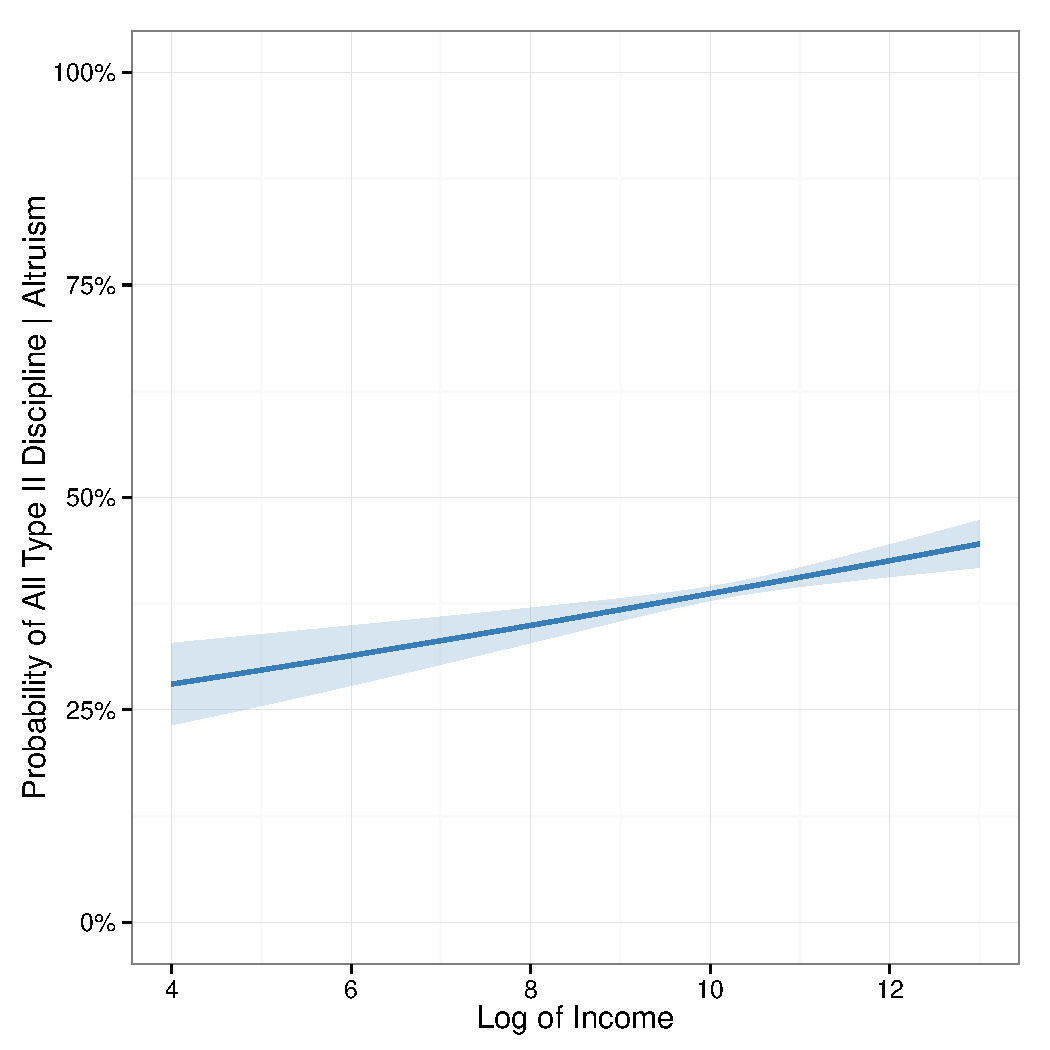
\includegraphics[width=\maxwidth]{ModelResultGph1-1} \caption[]{$P(\text{All } D_{II})$ as a function of $\log{y}$\label{modModelResultGph1}}
\end{figure}



\begin{figure}
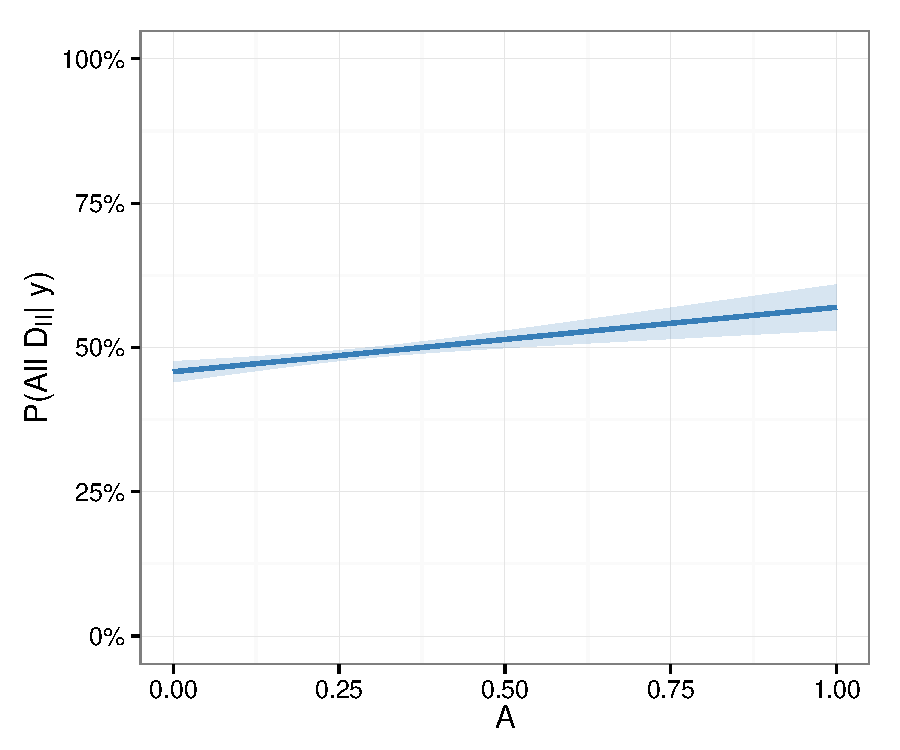
\includegraphics[width=\maxwidth]{ModelResultGph2-1} \caption[]{$P(\text{All } D_{II})$ as a function of $A$\label{modModelResultGph2}}
\end{figure}




\section{Discussion}\label{discussion}

The results of the analysis presented above confirm the hypothesis that
more altruistic households will tend to engage in ostensibly higher-cost parenting strategies
associated with wellbeing to a greater extent than less altruistic
households. This effect of altruism observed above is independent of the
income effect observed by other researchers. To the extent that the
other assumptions of the theoretical model hold, the results of this
analysis suggest that relatively simple models of human behavior might
be able to explain how families become involved with the child welfare
system.

What should be clear to the reader at this point is that the model
developed and tested in this manuscript is implicitly defining child
maltreatment as a problem of poverty. While previous researchers have
certainly drawn the connection between child welfare and poverty, such
literature usually attempts to examine the link between poverty and
deviant parental behaviors. Here, an alternative approach is taken in
defining maltreatment based on the manner in which poverty effects a
given child (in terms of their well-being) and the biological and social
context from which the parental behaviors emanate (resource constraints
and level of parental altruism).

In defining maltreatment in this manner, this manuscript breaks from
established lines of thinking about child maltreatment. Indeed, many
statutes specifically preclude poverty and homelessness as factors to be
considered when making legal determinations as to whether or not a given
child has been maltreated. The model presented here also elucidates the dynamic nature
of households and the variety of potential intervention points available
to the child welfare social work community.

\section{Limitations and Future
Directions}\label{limitations-and-future-directions}

Despite the usefulness of the model, it does suffer from an implicit
assumption of a parent who desires to invest (at least some) resources
in their child. The model presented here would suggest that all parents
would have a propensity to harm their children under a certain mix of
altruism and resource constraints, but that they typically seek to make
investments in children which maximize the child's utility subject to the utility of other household members. However,
some parents suffer from various forms of psychopathology which may
yield a desire to harm children under any circumstances. Instances of
pedophilic sadism seem to be evidence that such individuals do exist.
For those individuals, a model of maltreatment focused on the \citet{Kempe1962} ``defect of character'' seems
more appropriate than the one presented here. The point of this
manuscript, however, is that there is no reason to believe that such
individuals are a normal part of society or even a normal part of the
Western child welfare system. Such individuals likely represent the
margins of both populations and policies and interventions should be
developed with this theoretical framework in mind.

The analysis presented here is consistent with a resource constraint
theory of child maltreatment. However, the available data did not allow
for a direct test of all aspects of the model. A direct test of the
model would require information on how much parents prefer one form of
discipline to another given the relative monetary or cognitive ``costs''
or ``benefits'' of a given strategy and how these preferences vary as a
function of resource constraints. Specifically, future research could
explore the line of experiments conducted by \citet{Greene2014}. One
could, for example, imagine a brain-imaging experiment in which
parent-subjects were placed under cognitive load and asked to make
decisions about various parenting strategies. Understanding how
parenting decisions are made within the dual-process theory of morality
(or a similar framework) seems critical to the understanding of
maltreatment. Additional research could be undertaken to properly
monetize various parenting strategies and specifically test the
assumption that more resource intensive parenting strategies tend to
increase the wellbeing of children.

From a social service practice perspective, the results of this analysis suggest that
some families may be helped more by increases in income or other
concrete resources than the sorts of psychotherapeutic interventions
which tend to be prevalent in child welfare service plans. The study
does not refute the value of psychotherapeutic interventions. It does,
however, suggest that other forms of intervention may work better in
certain families. Although the BMA does exclude maternal frustration as
a covariate in the final selected model, the analysis does not imply
that such factors (including forms of psychopathology) could play a
causal role in a parent's level of altruism or wealth. For those parents where
income is not a concern, this model would suggest that interventions
should focus on changing preferences (i.e.~altruism or caring and
sharing) of parents and households.

The results of the BMA presented here also deserve more detailed
examination. Although the BMA suggests a final model which excludes many
of the control variables which would typically be included in a
statistical model of parenting behavior (e.g.~age, race, gender, etc.),
the BMA does not rule out the possibility that such demographic
variables may play a causal role in altruism per se. Such a question
could be further explored through a multiple equation model (e.g.~path
analysis, etc.). Finally, additional research is needed (through the
direct study of child protective services workers, family law judges or other means) to understand the
societal variability of the wellbeing threshold. In other words, since
the model presented here proceeds from the assumption that the wellbeing
threshold is societally defined, research should be conducted to help
the field understand precisely how the threshold varies within and
between countries throughout the world; both presently and across time.


% \begin{acknowledgements}
% This research was completed in 
% \end{acknowledgements}

% BibTeX users please use one of
%\bibliographystyle{spbasic}      % basic style, author-year citations
%\bibliographystyle{spmpsci}      % mathematics and physical sciences
%\bibliographystyle{spphys}       % APS-like style for physics
%\bibliography{}   % name your BibTeX data base

% % Non-BibTeX users please use
\begin{thebibliography}{50}
\providecommand{\natexlab}[1]{#1}
\providecommand{\url}[1]{{#1}}
\providecommand{\urlprefix}{URL }
\expandafter\ifx\csname urlstyle\endcsname\relax
  \providecommand{\doi}[1]{DOI~\discretionary{}{}{}#1}\else
  \providecommand{\doi}{DOI~\discretionary{}{}{}\begingroup
  \urlstyle{rm}\Url}\fi
\providecommand{\eprint}[2][]{\url{#2}}

\bibitem[{Baumrind(1993)}]{Baumrind1993}
Baumrind D (1993) The average expectable environment is not good enough: A
  response to scarr. Child Development 64(5):1299--1317

\bibitem[{Baumrind(1995)}]{Baumrind1995}
Baumrind D (1995) Child maltreatment and optimal caregiving in social contexts.
  Garland Publishing

\bibitem[{Becker(1981)}]{Becker1981}
Becker GS (1981) A Treatise on the Family. Harvard university press

\bibitem[{Belsky et~al(1991)Belsky, Steinberg, and Draper}]{Belsky1991}
Belsky J, Steinberg L, Draper P (1991) Childhood experience, interpersonal
  development, and reproductive strategy: An evolutionary theory of
  socialization. Child development 62(4):647--670

\bibitem[{Berger et~al(2008)Berger, Brooks-Gunn, Paxson, and
  Waldfogel}]{Berger2008}
Berger L, Brooks-Gunn J, Paxson C, Waldfogel J (2008) First-year maternal
  employment and child outcomes: Differences across racial and ethnic groups.
  Children and Youth Services Review 30(4):365--387

\bibitem[{Berger(2007)}]{Berger2007}
Berger LM (2007) Socioeconomic factors and substandard parenting. Social
  Service Review 81(3):485--522

\bibitem[{Berger and Waldfogel(2004)}]{BergerAndWoldfogel2004}
Berger LM, Waldfogel J (2004) Out-of-home placement of children and economic
  factors: An empirical analysis. Review of Economics of the Household
  2(4):387--411

\bibitem[{Berger et~al(2009)Berger, Paxson, and Waldfogel}]{Berger2009}
Berger LM, Paxson C, Waldfogel J (2009) Income and child development. Children
  and Youth Services Review 31(9):978--989

\bibitem[{Blundell et~al(2007)Blundell, Chiappori, Magnac, and
  Meghir}]{Blundell2007}
Blundell R, Chiappori PA, Magnac T, Meghir C (2007) Collective labour supply:
  Heterogeneity and non-participation. The Review of Economic Studies
  74(2):417--445

\bibitem[{Brandon(1999)}]{Brandon1999}
Brandon PD (1999) The state, the child, and imperfect parenting. Rationality
  and Society 11(4):399--418

\bibitem[{Brandon(2001)}]{Brandon2001}
Brandon PD (2001) State intervention in imperfect families: The child, the
  state, and imperfect parenting reconsidered from a theory of caomparative
  advantage. Rationality and Society 13(3):285--303

\bibitem[{Burgess and Conger(1978)}]{Burgess1978}
Burgess RL, Conger RD (1978) Family interaction in abusive, neglectful, and
  normal families. Child development pp 1163--1173

\bibitem[{Cameron and Freymond(2006)}]{Cameron2006}
Cameron G, Freymond N (2006) Towards positive systems of child and family
  welfare: International comparisons of child protection, family service, and
  community caring systems. University of Toronto Press

\bibitem[{Cancian et~al(2013)Cancian, Yang, and Slack}]{Cancian2013}
Cancian M, Yang MY, Slack KS (2013) The effect of additional child support
  income on the risk of child maltreatment. Social Service Review
  87(3):417--437

\bibitem[{Chagnon(1983)}]{Chagnon1983}
Chagnon NA (1983) Yanomam{\"o}: The Fierce People. New York: Holt, Rinehart and
  Winston. 1991 Yanomam{\"o}: The Last Days of Eden. San Diego: Harcourt Brace

\bibitem[{Chiappori(1988)}]{Chiappori1988}
Chiappori PA (1988) Rational household labor supply. Econometrica: Journal of
  the Econometric Society pp 63--90

\bibitem[{Courtney et~al(2005)Courtney, Dworsky, Piliavin, and
  Zinn}]{Courtney2005}
Courtney ME, Dworsky A, Piliavin I, Zinn A (2005) Involvement of tanf applicant
  families with child welfare services. Social Service Review 79(1):119--157

\bibitem[{Daly and Wilson(1988)}]{Daly1988}
Daly M, Wilson M (1988) Homicide. Transaction Publishers

\bibitem[{Dawkins(1976)}]{Dawkins1976}
Dawkins R (1976) The selfish gene. Oxford university press

\bibitem[{Donni and Chiappori(2011)}]{Chiappori2011}
Donni O, Chiappori PA (2011) Nonunitary models of household behavior: A survey
  of the literature. In: Household economic behaviors, Springer, pp 1--40

\bibitem[{Fein and Lee(2003)}]{Fein2003}
Fein DJ, Lee WS (2003) The impacts of welfare reform on child maltreatment in
  delaware. Children and Youth Services Review 25(1):83--111

\bibitem[{Gershoff(2002)}]{Gershoff2002}
Gershoff ET (2002) Corporal punishment by parents and associated child
  behaviors and experiences: a meta-analytic and theoretical review.
  Psychological bulletin 128(4):539

\bibitem[{Gil(1970)}]{Gil1970}
Gil DG (1970) Violence against children: Physical child abuse in the United
  States. Harvard University Press Cambridge, MA

\bibitem[{Gorman(1976)}]{Gorman1976}
Gorman WM (1976) Tricks with utility functions. Essays in economic analysis pp
  211--243

\bibitem[{Greene(2014)}]{Greene2014}
Greene JD (2014) Beyond point-and-shoot morality: Why cognitive (neuro) science
  matters for ethics. Ethics 124(4):695--726

\bibitem[{Hamilton(1964)}]{Hamilton1964}
Hamilton WD (1964) The genetical evolution of social behaviour. i. Journal of
  theoretical biology 7(1):1--16

\bibitem[{Ho et~al(2014)Ho, Konrath, Brown, and Swain}]{Ho2014}
Ho SS, Konrath S, Brown S, Swain JE (2014) Empathy and stress related neural
  responses in maternal decision making. Decision Neuroscience 8:152

\bibitem[{Hoeting et~al(1999)Hoeting, Madigan, Raftery, and
  Volinsky}]{Hoeting1999}
Hoeting JA, Madigan D, Raftery AE, Volinsky CT (1999) Bayesian model averaging:
  a tutorial. Statistical science pp 382--401

\bibitem[{Kempe et~al(1962)Kempe, Silverman, Steele, and
  Droegmuellar}]{Kempe1962}
Kempe C, Silverman F, Steele B, Droegmuellar W (1962) The battered child
  syndrome. The Journal of American Medical Association 181:4--11

\bibitem[{Mani et~al(2013)Mani, Mullainathan, Shafir, and Zhao}]{Mani2013}
Mani A, Mullainathan S, Shafir E, Zhao J (2013) Poverty impedes cognitive
  function. science 341(6149):976--980

\bibitem[{Milner(1998)}]{Milner1998}
Milner LS (1998) Hardness of heart/hardness of life: the stain of human
  infanticide. University Press of America

\bibitem[{Nelson(1986)}]{Nelson1986}
Nelson BJ (1986) Making an issue of child abuse: Political agenda setting for
  social problems. University of Chicago Press

\bibitem[{Paxson and Waldfogel(2002)}]{Paxson2002}
Paxson C, Waldfogel J (2002) Work, welfare, and child maltreatment. Journal of
  Labor Economics 20(3):435--474

\bibitem[{Paxton et~al(2012)Paxton, Ungar, and Greene}]{Paxton2012}
Paxton JM, Ungar L, Greene JD (2012) Reflection and reasoning in moral
  judgment. Cognitive Science 36(1):163--177

\bibitem[{Pelton(1981)}]{Pelton1981}
Pelton LH (1981) The social context of child abuse and neglect. Human Sciences
  Press New York

\bibitem[{Pelton(1994)}]{Pelton1994}
Pelton LH (1994) The role of material factors in child abuse and neglect.
  Protecting children from abuse and neglect: Foundations for a new national
  strategy pp 131--181

\bibitem[{Plomin et~al(1994)Plomin, Owen, and McGuffin}]{Plomin1994}
Plomin R, Owen MJ, McGuffin P (1994) The genetic basis of complex human
  behaviors. Science 264(5166):1733--1739

\bibitem[{Raftery et~al(2009)Raftery, Hoeting, Volinsky, Painter, and
  Yeung}]{Raftery2009}
Raftery A, Hoeting J, Volinsky C, Painter I, Yeung KY (2009) Bma: Bayesian
  model averaging. r package version 3.12. URL: http://CRAN R-project
  org/package= BMA

\bibitem[{Regalado et~al(2004)Regalado, Sareen, Inkelas, Wissow, and
  Halfon}]{Regalado2004}
Regalado M, Sareen H, Inkelas M, Wissow LS, Halfon N (2004) Parents' discipline
  of young children: Results from the national survey of early childhood
  health. Pediatrics 113(Supplement 5):1952--1958

\bibitem[{Ridley(2003)}]{Ridley2003}
Ridley M (2003) Nature via nurture: Genes, experience, and what makes us human.
  HarperCollins Publishers

\bibitem[{Roy(1947)}]{Roy1947}
Roy R (1947) La distribution du revenu entre les divers biens. Econometrica,
  Journal of the Econometric Society pp 205--225

\bibitem[{Russell and Trainor(1984)}]{Russell1984}
Russell AB, Trainor CM (1984) Trends in child abuse and neglect: A national
  perspective. American Humane Association, Children's Division

\bibitem[{Sedlak and Broadhurst(1996)}]{Sedlak1996}
Sedlak AJ, Broadhurst DD (1996) The national incidence study of child abuse and
  neglect. Washington DC US Department of Health and Human Services

\bibitem[{Slack et~al(2007)Slack, Lee, and Berger}]{Slack2007}
Slack KS, Lee BJ, Berger LM (2007) Do welfare sanctions increase child
  protection system involvement? a cautious answer. Social Service Review
  81(2):207--228

\bibitem[{Sodian et~al(2004)Sodian, Schoeppner, and Metz}]{Sodian2004}
Sodian B, Schoeppner B, Metz U (2004) Do infants apply the principle of
  rational action to human agents? Infant Behavior and Development 27(1):31--41

\bibitem[{Stith et~al(2009)Stith, Liu, Davies, Boykin, Alder, Harris, Som,
  McPherson, and Dees}]{Stith2009}
Stith SM, Liu T, Davies LC, Boykin EL, Alder MC, Harris JM, Som A, McPherson M,
  Dees J (2009) Risk factors in child maltreatment: A meta-analytic review of
  the literature. Aggression and violent behavior 14(1):13--29

\bibitem[{Stuebe et~al(2010)Stuebe, Kleinman, Gillman, Rifas-Shiman, Gunderson,
  and Rich-Edwards}]{Stuebe2010}
Stuebe AM, Kleinman K, Gillman MW, Rifas-Shiman SL, Gunderson EP, Rich-Edwards
  J (2010) Duration of lactation and maternal metabolism at 3 years postpartum.
  Journal of Women's Health 19(5):941--950

\bibitem[{Suter and Hertwig(2011)}]{Suter2011}
Suter RS, Hertwig R (2011) Time and moral judgment. Cognition 119(3):454--458

\bibitem[{Taylor et~al(2010)Taylor, Manganello, Lee, and Rice}]{Taylor2010}
Taylor CA, Manganello JA, Lee SJ, Rice JC (2010) Mothers' spanking of
  3-year-old children and subsequent risk of children's aggressive behavior.
  Pediatrics 125(5):e1057--e1065

\bibitem[{Trivers(1974)}]{Trivers1974}
Trivers RL (1974) Parent-offspring conflict. American zoologist 14(1):249--264

\end{thebibliography}
% \bibliographystyle{spbasic}
% \bibliography{qualpaper_v5}

\end{document}
% end of file template.tex

